\documentclass[12pt,oneside,a4paper,chapter=TITLE,english,brazil,sumario=abnt-6027-2012]{abntex2}

\usepackage{../sub/tcc_style}

\titulo{\bfseries MATRIZ DE CORRELAÇÃO ENTRE AS QUATRO PRINCIPAIS LIGAS DE ESPORTES DOS ESTADOS UNIDOS}

\autor{GUILHERME DE MORAES MASUKO}



\local{RIO DE JANEIRO/ RIO DE JANEIRO}
\data{\the\year}
\tipotrabalho{artigo}
\instituicao{Pontifícia Universidade Católica - Rio de Janeiro (PUC-Rio)}




\begin{document}
	
\clearpage\maketitle
\thispagestyle{empty}
\setlength{\absparsep}{18pt} 
\begin{resumo}
	
	A presente análise buscou estudar o comportamento entre a performance dos times na quatro ligas mais famosas dos Estados Unidos e Canadá. Conhecidas como "Big Four", as quatro ligas de esportes coletivos são a Major League Baseball (MLB), a National Basketball Association (NBA), a National Football League (NFL) e a National Hockey League (NHL). Foi utilizado o coeficiente de correlação de Pearson, como medidor da relação entre a performance desses times e as regiões metropolitanas como indexador. O resultado final do trabalho conta com uma matriz de correlação medindo a relação entre a performance média dos times das regiões metropolitanas em seus pares de esportes. Um resultado de destaque foi a correlação entre as ligas NBA e NHL, onde constatou uma correlação de 0,76.
	\noindent
	
	\textbf{Palavras-chave}:  Correlação. Esporte.   
\end{resumo}


	
	\pdfbookmark[0]{\contentsname}{toc}
	\tableofcontents*
	\cleardoublepage
	
	
	
	\textual 
	\pagestyle{simple}
	\aliaspagestyle{chapter}{simple}
	
\chapter{Introdução}

	Os Estados Unidos é um país conhecido pelo seu ótimo desempenho no esporte. As quatro principais ligas esportivas profissionais nos Estados Unidos e Canadá, comumente referenciada como "Big Four", são as competições profissionais mais competitivas de esportes coletivos nesses países. As quatro ligas inclusas nessa definição são a Major League Baseball (MLB), a National Basketball Association (NBA), a National Football League (NFL) e a National Hockey League (NHL). É comum verificar que vários times entre as ligas Big Four estão situados em mesma região metropolitana.
	
	O presente estudo objetivou-se em questionar as relações que se têm entre estas regiões metropolitanas e a performance média obtida por seus times. Utilizando o coeficiente de correlação de Pearson, foi medida a correlação entre a população destas regiões com a performance média de seus times. O coeficiente de Pearson, como mostra em \citeonline{corr_pearson}, pode ter valores entre -1 e 1. Um resultado muito próximo de um nos diria que uma região metropolitana com grande população está ligada à boas performances médias, enquanto regiões com baixa população estão ligadas à performances médias menos regulares. Já um resultado próximo de menos um nos entregaria uma inferência inversa à acima.
	
	Para o restante do trabalho, foi estudado o relacionamento que se têm entre a performance média das regiões metropolitanas entre pares de esporte. Isto é, queremos saber qual o comportamento dos times de mesma região metropolitana, mas em esportes diferentes. Por exemplo, queremos descobrir se os times da NHL da região metropolitana de New York City, New Jersey Devils, New York Islanders e New York Rangers, tem performance média parecida com os times New York Knicks e Brooklyn Nets da liga de basquete.
	


\chapter{Metodologia}

	Para mensurar a relação entre a performance média das regiões metropolitanas nas ligas norte-americana NBA, MLB e NFL, será proposto como medidor de performance, visualizado na equação \ref{perf}, a razão entre vitórias e jogos de cada time, ou seja
	
	\begin{equation}
		P_i = \frac{W_i}{G_i}
		\label{perf}
	\end{equation}
	onde $P_i$ é a performance do time $i$, $W_i$ é a quantidade de vitórias na temporada regular do time $i$ e $G_i$ é a quantidade de jogos da temporada regular do time $i$.
	
	Para a liga NHL, como há um esquema de pontuação diferente, onde o time ganha dois pontos caso vença, um ponto caso seja derrotado em um overtime, e zero caso seja derrotado no tempo normal, o medidor de performance é proposto a partir da razão entre pontuação do time e pontuação possível, este último travado em 164 (pontuação caso um time ganhar as 82 partidas que contém uma temporada regular). A equação \ref{perf_nhl} ilustra isso.
	
	\begin{equation}
		P_i = \frac{Pt_i}{maxPt} = \frac{Pt_i}{164}
		\label{perf_nhl}
	\end{equation}
	onde $P_i$ é a performance do time $i$, $Pt_i$ é a pontuação na temporada regular do time $i$ e $maxPt$ é a pontuação máxima, de 164 pontos, da temporada regular que um time pode atingir.
	
	Algumas ligas possues divisões de localidades para que seja possível manter a quantidade de jogos da temporada regular. O presente estudo não discriminará em qual divisão cada time pertence, fazendo apenas uma agregação simples da performance de cada time, considerando que essas divisões mantém o mesmo nível de dificuldade.
	
	Possivelmente vários times podem estar situados em mesma região metropolitana e para chegar na performance da região será utilizado a média simples da performance de cada time.
	
	E, finalmente, para mensurar a relação entre a performance média das regiões metropolitanas usaremos a matriz de correlação para as quatro principais ligas norte-americanas. Como pode ser visto em \citeonline{corr}, correlação é uma medida estatística de relação (causal ou não-causal) entre duas variáveis abordando o comportamento da relação entre elas. O coeficiente de correlação utilizado pela presenta análise será o de Pearson, o coeficiente de correlação mais comumente usado. 
	
	O coeficiente de correlação de Pearson, segundo \citeonline{corr_pearson}, define o quanto e em qual direção duas variáveis estão relacionadas, sendo obtida a partir da seguinte fórmula demonstrada na equação \ref{corr} abaixo.. Usado normalmente como $\rho$, o coeficiente pode ter valores em um range de $-1$ à $1$, isto é, $-1 \leq \rho \leq 1$, onde $\rho =-1$ significa uma relação perfeitamente negativa entre as variáveis, $\rho=1$ uma relação perfeitamente positiva, e $\rho=0$ uma relação de não dependência linear (isso não diz nada sobre não haver dependência de modo geral entre as variáveis).
	
	\begin{equation}
		\rho_{X,Y} = \frac{\mbox{COV}(X,Y)}{\sqrt{\mbox{VAR}(X)}\sqrt{\mbox{VAR}(X)}}
		\label{corr}
	\end{equation}
	onde $\rho_{X,Y}$ é a correlação entre $X$ e $Y$.
	
	A matriz de correlação é uma ferramente estatística capaz de medir a correlação de uma coleção de variáveis em seus pares, uma ótima maneira de obter de forma reduzida, o comportamento de várias séries em uma só tabela. Uma matriz de correlação de $n$ variáveis $X_1$,...,$X_n$, é uma matriz $nxn$, no qual o $i$,$j$-ésimo elemento da matriz é a correlação entre $X_i$ e $X_j$, isto é, $\rho_{X_i,X_j}$.
	
	
\chapter{Dados}

	Os dados das regiões metropolitanas dos Estados Unidos e Canadá utilizados nesse estudo foram obtidos através de \citeonline{reg_metro}, onde uma tabela pode ser encontrada relacionando cada região metropolitana com os times da big four. Nesta tabela também há informações sobre a quantidade populacional de cada região, com dados atualizados para o ano de 2016.
	
	A primeira liga abordada foi a National Hockey League. Para esta e todas as demais ligas presentes neste trabalho, foi escolhido os resultados da temporada regular de 2018. No gráfico \ref{nhl}, podemos verificar a performance de cada time na temporada regular utilizando o medidor proposto em particular à esta liga, como a razão entre a pontuação do time sobre a máxima pontuação possível. A liga é divida entre quatro divisões, são elas a do Atlântico, Metropolitana, Central e do Pacífico.
	
	\begin{figure}[H]
		\centering
		\caption{Performance Temporada Regular National Hockey League (NHL) 2018}
		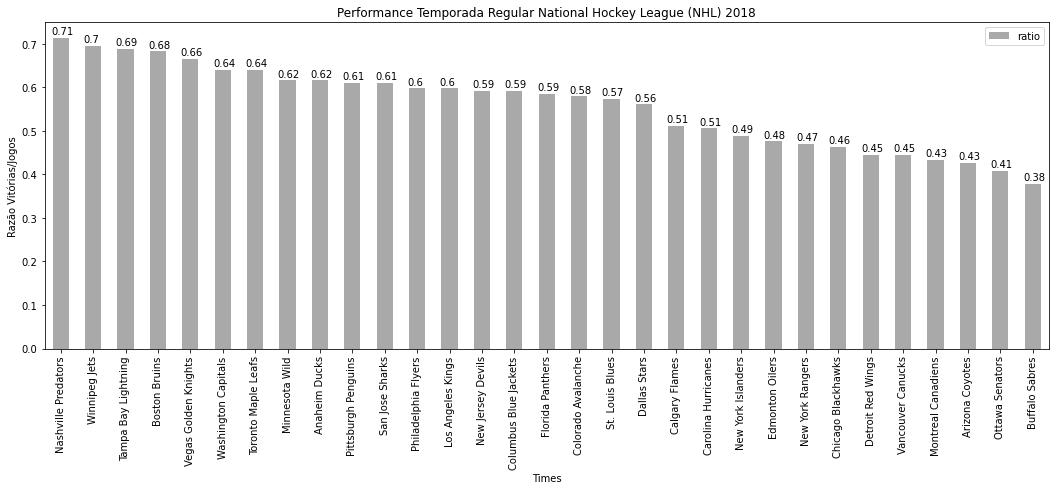
\includegraphics[scale=0.4]{../../output/figures/nhl.png}
		\label{nhl}
		\\ \vspace{0.25cm}
		\raggedright
		\footnotesize{Fonte: Elaboração própria a partir de \citeonline{nhl}}
	\end{figure}
	
	O destaque para a liga de hóquei ficou para o Nashville Predators. O time de Nashville se mostrou muito forte com uma razão de 71\% de performance na temporada regular, mas mesmo assim acabou caindo na segunda rodada dos playoffs para o Winnipeg Jets, este com a segunda melhor campanha na temporada regular, com 70\% de performance. Por fim, o time que acabou sendo campeão foi o Washington Capitals.
	
	Para as ligas restantes o estimador de performance é obtido a partir da equação \ref{perf}. O segundo esporte analisado é o basquete. Utilizando dados da temporada regular da National Basketball Association, pode se ver a lista de times e suas respectivas performance através do gráfico \ref{nba}. A NBA é dividida em duas divisões, conhecidas como Conferências Leste e Oeste.
	
	\begin{figure}[htbp]
		\centering
		\caption{Performance Temporada Regular National Basketball Association (NBA) 2018}
		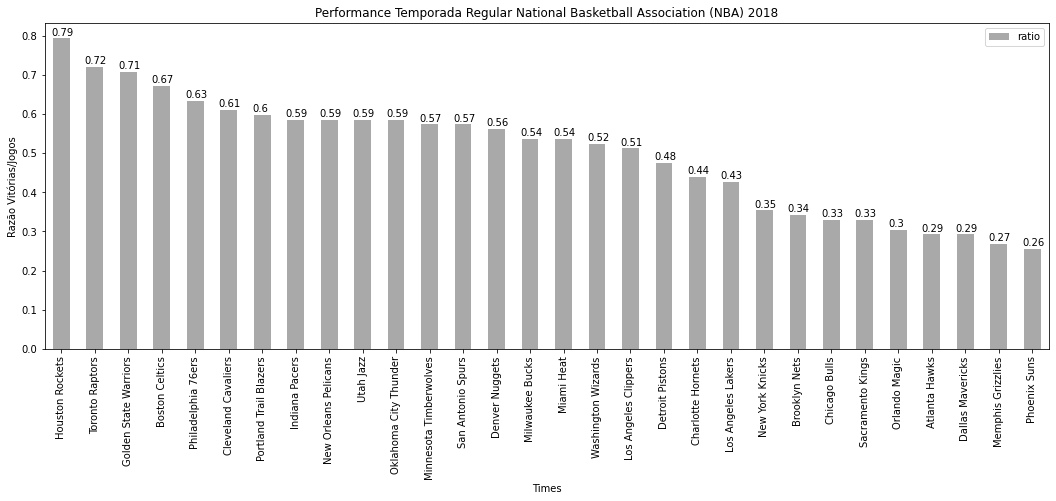
\includegraphics[scale=0.4]{../../output/figures/nba.png}
		\label{nba}
		\\ \vspace{0.25cm}
		\raggedright
		\footnotesize{Fonte: Elaboração própria a partir de \citeonline{nba}}
	\end{figure}
	
	Com destaque para o time Houston Hockets, o time obteve 65 vitórias. Mesmo com a tamanha regularidade na temporada, com 79\% em performance, o time caiu diante do Golden State Warriors, nas finais da Conferência Oeste. O time da região metropolitana de San Francisco Bay Area se sagrou campeão vencendo também a final da NBA sobre o Cleveland Cavaliers.
	
	A terceira liga é a Major League Baseball. O gráfico \ref{mlb} mostra a superioridade do time Boston Red Sox durante a temporada regular. O time também foi o campeão dos playoffs neste ano.
	
	\begin{figure}[htbp]
		\centering
		\caption{Performance Temporada Regular Major League Baseball (MLB) 2018}
		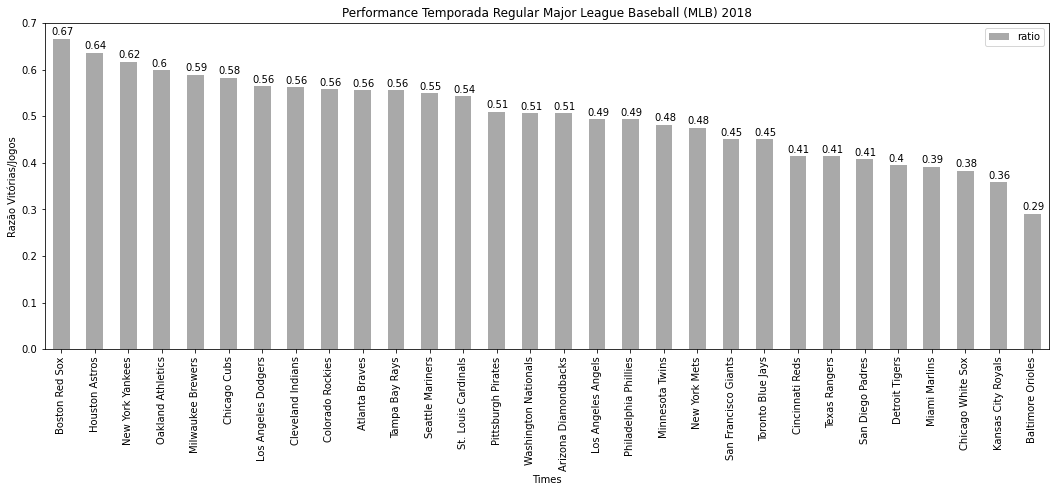
\includegraphics[scale=0.4]{../../output/figures/mlb.png}
		\label{mlb}
		\\ \vspace{0.25cm}
		\raggedright
		\footnotesize{Fonte: Elaboração própria a partir de \citeonline{mlb}}
	\end{figure}
	
	
	A quarta e última liga abordada nesse trabalho é a National Football League. 
	
	\begin{figure}[H]
		\centering
		\caption{Performance Temporada Regular National Football League (NFL) 2018}
		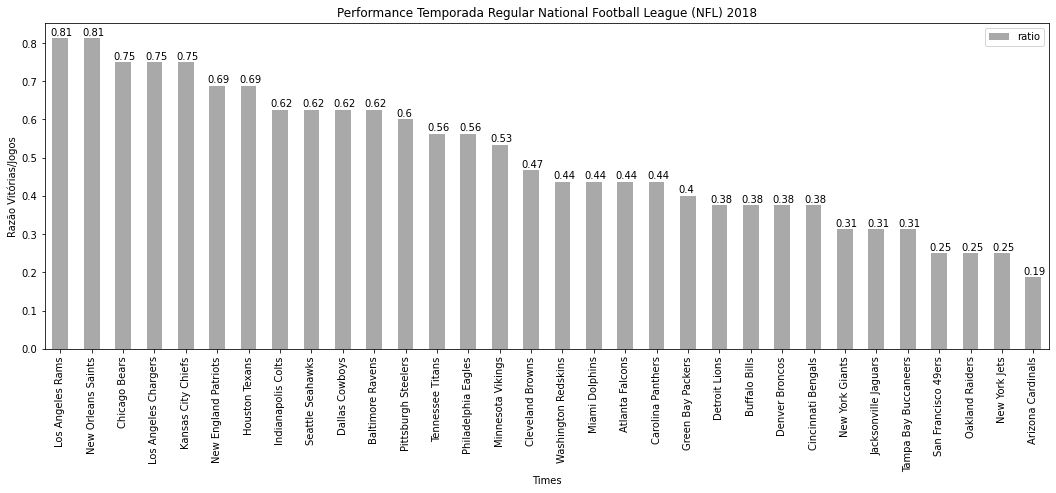
\includegraphics[scale=0.4]{../../output/figures/nfl.png}
		\label{nfl}
		\\ \vspace{0.25cm}
		\raggedright
		\footnotesize{Fonte: Elaboração própria a partir de \citeonline{nfl}}
	\end{figure}
	
	Mesmo que os times Los Angeles Rams e New Orleans Saints tivessem atingido a incrível marca de 81\% de performance na temporada regular como aponta o gráfico \ref{nfl}, o time que acabou como campeão de um dos eventos esportivos mais famosos conhecido como Super Bowl, foi o New Englands Patriots.

	
\chapter{Conclusão}

	Os primeiros resultados obtidos neste trabalho foram em relação a variável indexadora. Foi estimada a correlação entre a população de cada região metropolitana e a performance de seus respectivos times para cada liga. Os resultados são verificados na tabela \ref{tab:corr_table}.
	
	\begin{table}[H]
	\centering
	\caption{Correlação entre População e Performance média da Região Metropolitana para cada Liga}
	\begin{tabular}{lr}\hline
	& População (2016) \\\hline
	NFL & 0.004922 \\
	NBA & -0.176572 \\
	NHL & 0.006519 \\
	MLB & 0.150277 \\\hline
	\end{tabular}
	\label{tab:corr_table}
	\\ \vspace{0.25cm}
	\raggedright
	\footnotesize{Fonte: Elaboração própria.}
	\end{table}

	Os resultados mostram que para as ligas NFL e NHL, os níveis de correlação foram muito próximos de zero, podendo dizer que não há uma relação linear entre a performance média das regiões metropolitanas nestes esportes e a população destas regiões. Para o basquete, a correlação entre a performance média das regiões metropolitanas na NBA e a população é menor que zero, isso demonstra que há uma relação negativa entre essas duas variáveis. Enquanto que para a MLB, a relação entre estas duas variáveis foi positiva, mostrando que uma população maior está positivamente relacionada com a performance média de uma determinada região metropolitana. Embora existam essas relações para NBA e MLB, os coeficientes de correlação não foram grandes o suficiente para encontrar casos distintos ao que foi inferido.
	
	A matriz de correlação, visualizada na tabela \ref{tab:corr_matrix}, mostra a relação que se teve entre a performances média das regiões metropolitanas aos pares de ligas esportivas.

	\begin{table}[H]
	\centering
	\caption{Matriz de Correlação da Performance média da Região Metropolitana entre as Ligas}
	\begin{tabular}{lrrrr}
	& NFL & NBA & NHL & MLB \\\hline
	NFL &  & 0.237000 & 0.304000 & -0.050000 \\\hline
	NBA & 0.237000 &  & 0.760000 & 0.325000 \\\hline
	NHL & 0.304000 & 0.760000 &  & 0.432000 \\\hline
	MLB & -0.050000 & 0.325000 & 0.432000 &  \\\hline
	\end{tabular}
	\label{tab:corr_matrix}
	\\ \vspace{0.25cm}
	\raggedright
	\footnotesize{Fonte: Elaboração própria.}
	\end{table}	

	O basquete e o hóquei foram dois esportes em destaque, onde a performance média das regiões metropolitanas dos times se mostraram positivamente correlacionados com um coeficiente relativamente alto. Isso mostra que times de mesma região metropolitana devem ter tido resultados mais parecidos. Esse não é o caso da correlação entre a NFL e MLB, onde o coeficiente de Pearson foi de -0,05.

	
	\bibliographystyle{abntex2-alf}
	\bibliography{ref}

\end{document}
	
	